\chapter{Introduction}
\label{ch:introduction}
Conventional energy resources such as fossil fuels and nuclear energy are not only limited but also pose adverse effects on the environment. Therefore, we are striving to find a cheap and renewable source of energy. Wind energy is such source of energy, getting more popular and more affordable. Novel wind turbine designs such as \indexAcron{Vertical-Axis Wind Turbine}{VAWT} are now a promising research field that can satisfy this growing demand.

	\begin{figure}[!b]
        \centering
        \begin{subfigure}[b]{0.25\textwidth}
                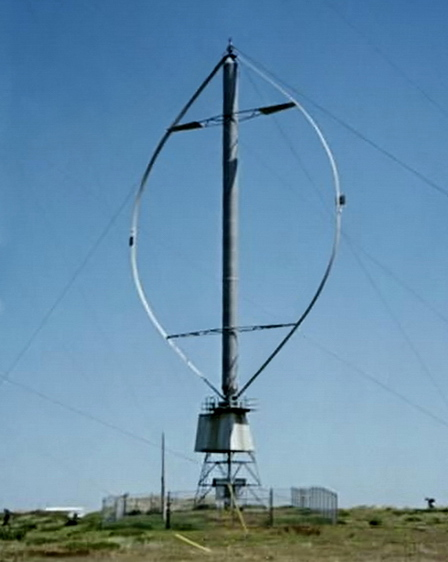
\includegraphics[height=0.2\textheight]{figures/introduction/Darrieus-windmill.jpg}
                \caption{VAWT: Darrieus wind turbine\cite{darrieusWindmill}}
                \label{fig:Darrieus-windmill}
        \end{subfigure}%
        \qquad \qquad%add desired spacing between images, e. g. ~, \quad, \qquad etc.
          %(or a blank line to force the subfigure onto a new line)
        \begin{subfigure}[b]{0.25\textwidth}
                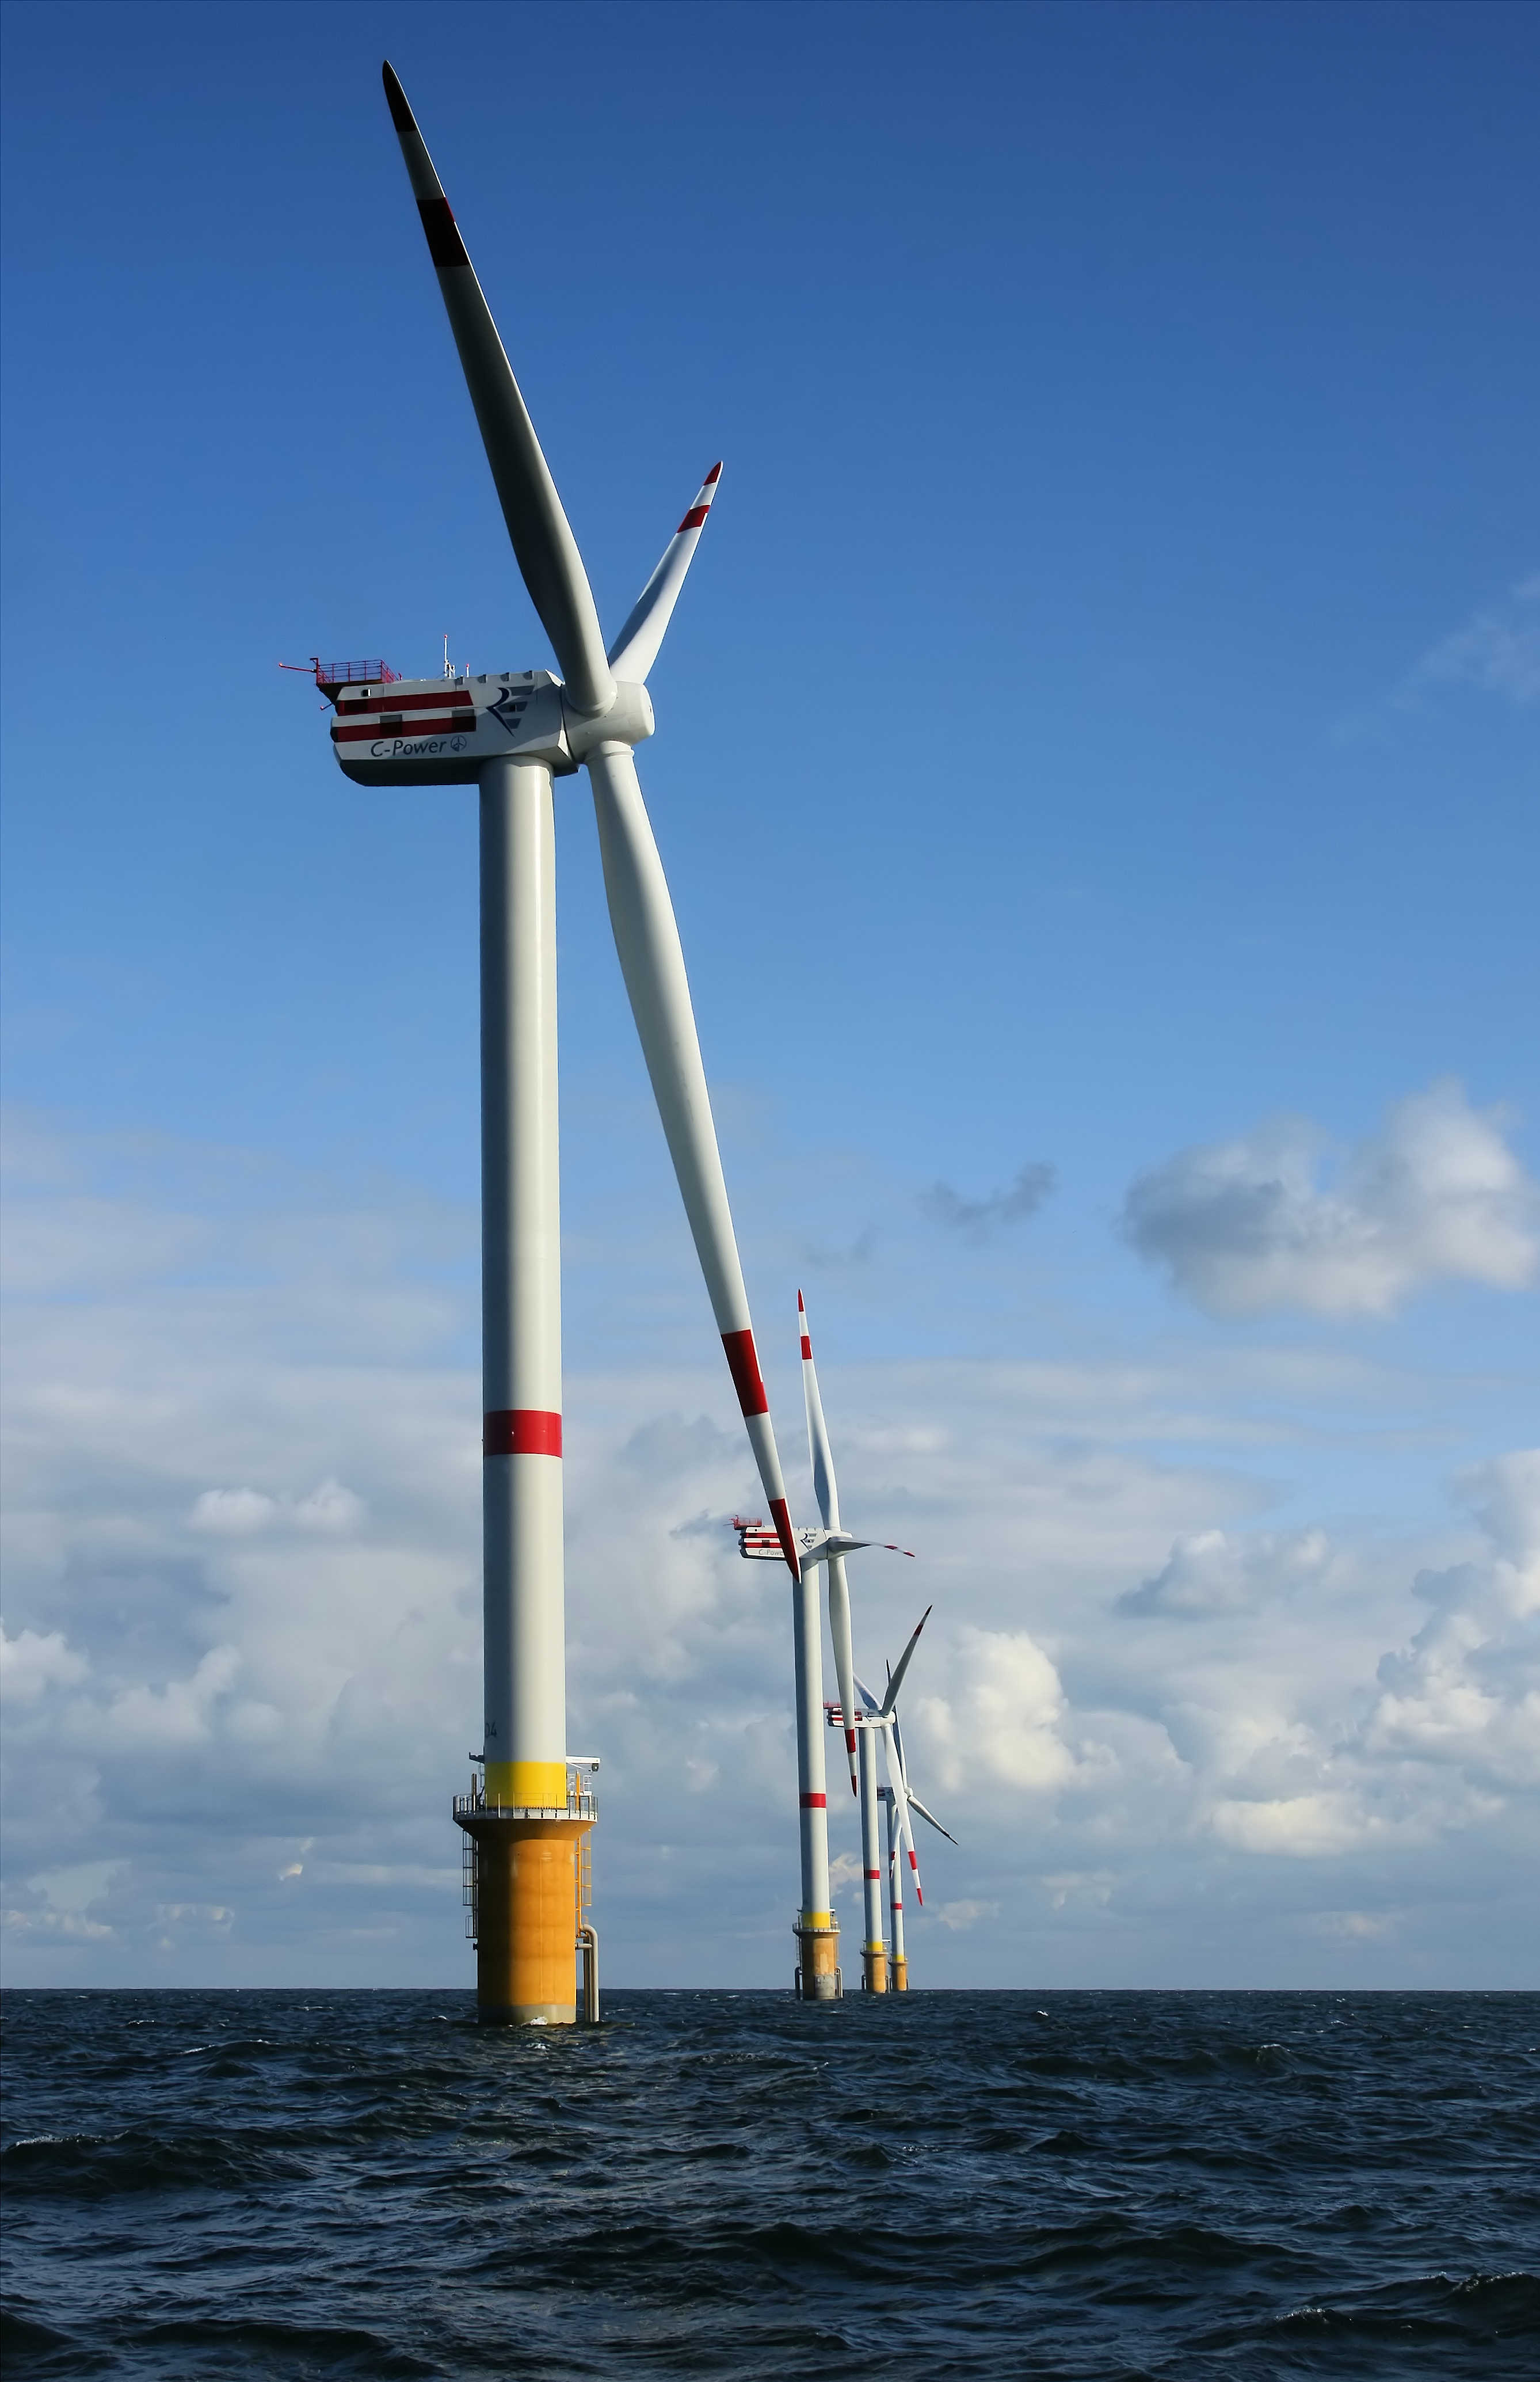
\includegraphics[height=0.2\textheight]{figures/introduction/HAWT_compressed.jpg}
                \caption{HAWT: Offshore wind turbine \cite{HAWTWindmill}}
                \label{fig:HAWT}
        \end{subfigure}
        \caption{VAWT vs. HAWT}
        \label{fig:VAWTvsHAWT}
	\end{figure}

VAWTs are unlike the normal wind turbines, which are mounted on a mast away from the ground and generate energy by spinning perpendicular to the ground, figure \ref{fig:VAWTvsHAWT}, whereas the \printAcron{Horizontal-Axis Wind Turbine}{VAWT}, spins parallel to the ground with its hub located at the ground, figure \ref{fig:HAWT}. The VAWT has it's generator located at the ground, allowing it to be easily accessible and maintained. However, the main advantage is the early wake dissipation of VAWTs. Near-wake experiments of Ferreira (2009) \cite{SimaoFerreira2009}, and simulations of Vermeer (2003) \cite{Vermeer2003a} have shown that the fluid past the turbine is more turbulent. Due to this higher turbulence, the flow is able to recover much earlier than convectional wind turbines. This allows the turbines to be placed much closer, potentially outputting more power per ground. Furthermore, VAWTs operate independently of the flow direction, and can operate at low wind speeds (i.e. at low tip-speed ratios).

However, there are some limitations that we must take into account. As the blades pass through their own wake, complex wake-body interactions take place, figure \ref{fig:3DunsteadyPanelVAWT}. These have adverse effects on the blade structure, making it more susceptible to fatigue. As the blade is constantly pitching, flow behaviors such as dynamic stall and constant vortex shedding take place \cite{SimaoFerreira2008a}. These complex fluid behaviors makes it hard to predict the performance of a VAWTs and this is one of the reasons why VAWTs are not widely used. 

	\begin{figure}[!t]
		\centering
		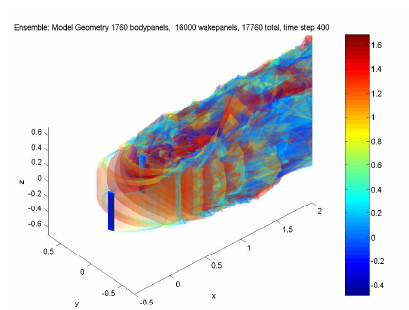
\includegraphics[width=0.6\linewidth]{figures/introduction/3DunsteadyPanelVAWT.png}
		\caption{3-D Unsteady Panel simulation of a Straight-bladed VAWT showing the strength of the shed vorticity. The VAWT blades interact with their own wake increasing the complexity of the wake geometry \cite{Dixon2008}}
		\label{fig:3DunsteadyPanelVAWT}
	\end{figure}

In addition, a VAWT operates at a large Reynolds, number making accurate numerical methods computationally very expensive. So we see that we require a numerical method that can not only reproduce accurate results, but is also efficient at modeling the flow around the turbine.

\section{Motivation and Goal}
The goal of this research is to develop an efficient, reliable, and accurate numerical method for modeling the flow around a \indexAcron{Two-Dimensional}{2-D} VAWT, enabling to compute the correct performance characteristics. The two approaches of investigating the flow around a turbine are by either using a numerical method to model the flow, or by performing an experimental test, for example in a wind tunnel.

To understand the unsteady aerodynamic behavior, \indexAcron{Particle Image Velocimetry}{PIV} has been a useful tool to visualize the flow around the turbine. PIV was used by Ferreira et al. (2007) \cite{Ferreira2007a}, showing that it is possible to measure the flow characteristics around the blade. The downside to experimental investigation is that it is very expensive to investigate all types of airfoil geometries, blade geometries and VAWT configurations. However, investigating this is vital in understanding the performance characteristics of VAWT. Furthermore, it is difficult to perform experiments on array of wind turbines in a wind tunnel.

Numerical methods are therefore a popular alternative as the cost of simulation is becoming progressively smaller, and the accuracy of the models are increasing day by day. \indexAcron{Actuator Disk}{AD} and \indexAcron{Blade Element Momentum}{BEM} models are the simplest models, built upon satisfying the momentum balance of the turbine with the fluid. The advantage is that they are very quick, however they lack the accuracy that are obtained by experimental simulation. Flow phenomenons such as dynamic stalls and flow separations cannot be modeled by these methods, and therefore we must rely on more powerful tools.

	\begin{figure}[!t]
		\centering
		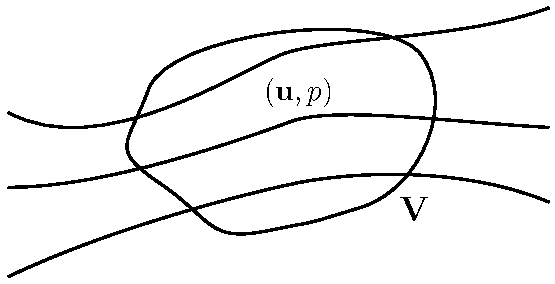
\includegraphics[width=0.4\linewidth]{figures/introduction/eulerianRF.pdf}
		\caption{Eulerian formulation of the fluid. We observe a given volume $\mathbf{V}$ and evaluate the change in properties of the fluid, velocity $\mathbf{u}$ and pressure $p$ at time passes.}
		\label{fig:eulerianRF}
	\end{figure}

To ensure more accuracy, one has to solve the Navier-Stokes equation of the flow around the turbine without large simplifications. \indexAcron{Computional Fluid Dynamics}{CFD} methods discretize the fluid into smaller cells (or volumes) and solve the Navier-Stokes equations. This type of formulation is known as an Eulerian formulation as we are evaluating the change in flow property in a given cell/volume, figure \ref{fig:eulerianRF}. In order to fully resolve the flow around the turbine, we would need a fine mesh near the blade where we have small scale vorticies. However, far from the body, where these vorticies dissipated into low frequency vortical structures, we can have lower mesh resolution. This means that at various regions of the flow, we require mesh resolutions of various magnitudes. This becomes a problem when we have moving boundaries as the mesh has to be adapted depending on the location of the body.

An alternative method is to use a Lagrangian formulation of the Navier-Stokes equations, known as vortex methods. These methods employ vorticity transport equations which makes them ideal for describing the evolution of the wake vorticity. Furthermore, they do not require cells/volumes to describe the domain. In addition, they use simulation acceleration methods such as \indexAcron{Fast Multipole Method}{FMM} and parallel computation in \indexAcron{Graphical Processing Units}{GPU} making them orders of magnitude faster than the typical CFD methods. However, vortex method cannot inherently take in account the solid body. They require additional methods that can describe the effect of the body in the fluid and the vorticity generated from the body.

	\begin{figure}[!t]
		\centering
		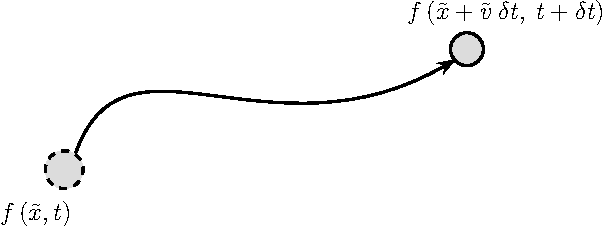
\includegraphics[width=0.4\linewidth]{figures/introduction/lagrangianRF2-crop.pdf}
		\caption{Lagrangian formulation of the fluid. We track the path of the individual fluid elements as time passes.}
		\label{fig:lagrangianRF}
	\end{figure}

We see that Eulerian method is accurate when describing the blade-wake interaction but not efficient when describing multi-scale domains. The Lagrangian method is very efficient in evolving the vorticity of the fluid. Due to auto-adaptive nature of the Lagrangian method, it is an ideal choice when describing the multi-scale flow characteristics. However, it is not efficient in resolving the near-body region, where the vorticity is generated. Therefore, in order to use the advantages of both methods, we have decided to use a domain-decomposition method, referred to as \indexAcron{Hybrid Eulerian-Lagrangian Vortex Particle Method}{HELVPM}. 

For the HELVPM, the Eulerian grid method will be used at the near-wall region of the blades, and the Lagrangian vortex method will be used in the wake region of the body. With proper coupling of these methods, we can ensure that this numerical method can capture not only the near-wake phenomena such as vortex shedding, dynamic stall, and the wake-body interaction, but also the large-scale flow structures such as the evolution of the VAWT wake.

\section{Research Aim and Plan}

We have formulated a research that can help us accomplish our goal. The research questions that are derived from the goal of the project is as follows:

\paragraph*{Research Questions:}
	\begin{itemize}
	\item \textit{Is it possible to develop an efficient and accurate numerical method by an
	hybrid approach, with the vortex particle method solving the wake, and the Navier-Stokes grid solver solving the near-body region?}
	
	\item \textit{Will it be able to predict similar performance characteristics and flow phenomena as observed from the experiments?}
	
	\item \textit{Will it be capable of simulating the blade-wake interaction and the dynamic stall?}
	
	\item \textit{Where are the errors and what are their sources?}
	\end{itemize}
%\textit{Is it possible to develop an efficient and accurate numerical method by an
%hybrid approach; where the vortex particle method is used in the wake, and the Navier-Stokes grid solver is
%used at the near-body region? Will it be able to simulate real life performance characteristics of a Vertical-Axis Wind Turbine? Will it be able to predict similar performance characteristics and flow phenomena as observed from the wind tunnel experimental setup? Will it be capable of simulating the blade-wake interaction
%and the dynamic stall? Where are the errors and what are their sources?}

In order to answer the research questions, the goal of the project is to develop an efficient and accurate numerical method that is not only capable of capturing the small scale flow phenomena such as the dynamic stall and the vortex shedding, but is also efficient at modeling the evolution of the wake. Once the model have been developed, we will verify the approach and validate it against cases obtained from literature.

\paragraph*{Research aim and plan:}
\textit{
	\begin{itemize}
	\item Develop the hybrid method for capturing small-scale phenomena and large scale phenomena.
	\item Verify the efficiency, reliability, and the accuracy of the model.
	\item Verify and validate the model with test cases from literature.
	\end{itemize}
}
The innovativeness of this project is that such hybrid modeling has not been yet applied for the wind energy problem case. Through the parallelization of the vortex particle method in a GPU and employing solver acceleration techniques such as the FMM, this simulation could give an edge in the understanding the flow behavior of a VAWT.

\section{Introduction to Hybrid Eulerian-Lagrangian Vortex \\Particle Method}

The \printAcron{Hybrid Eulerian-Lagrangian Vortex Particle Method}{HELVPM} is a domain decomposition method, where the Eulerian method and the Lagrangian method solves different regions of the fluid. The domain decomposition method simply splits the domain of interest and uses appropriate method in each domain. The Eulerian formulation will be used at the near-wall region, where we need proper description of the vorticity generation at the boundary, and the Lagrangian formulation is used away from the body, where we only need to evolve the vorticity field. Figure \ref{fig:domainDecomposition} shows the decomposition of the domain in the gridded and the non-gridded region.

Several studies have already been done: Cottet and Koumoutsakos (2000a)\cite{Cottet2000a}, Guermond and Lu (2000) \cite{Guermond2000a} simulated the advection dominated flows; Ould-Salhi et al. (2001) \cite{Ould-Salihi2001a} blended the finite difference and vortex method together; Winckelmans et al. (2005a) \cite{Winckelmans2005} investigated the trailing vorticies; Daeninck (2006) \cite{Daeninck2006} used a simplified coupling strategy, coupling Vortex Particle Method and Finite Diference Method; Stock (2010) \cite{Stock2010a} expanded Daeninck's strategy, coupling Vortex Particle Method and Finite Volume Method and modeled a 3-D rotor.

When evaluating the previous works, we see that not all domain decomposition methods are the same. The main difference between the methods is their coupling strategies. Most works employ the Schwartz alternating method to couple the vortex particle method and the grid solver. The Schwartz alternating method (or sometimes referred to as Schwartz iterative method), couples the vortex particle method and the grid solver by iteratively determining the boundary condition such that the stream functions in both domains, $\psi_L$ and $\psi_E$ in $\Omega_L$ and $\Omega_E$ respectively, match at the overlap region $\Omega_E-\Omega_L$, figure \ref{fig:domainDecomposition}. The summary of a single iteration of the Schwartz alternating method is as follows:
	\begin{itemize}
	\item Determine the Eulerian boundary condition, the stream function $\psi_{\Gamma_E}$ at the Eulerian boundary $\Gamma_E$, extracted from the Lagrangian stream function $\psi_L$in the Lagrangian subdomain $\Omega_L$.
	\item Solve for the stream function $\psi_E$ in the Eulerian subdomain $\Omega_E$ with the new boundary condition $\Gamma_E$.
	\item Determine the Lagrangian condition, the stream function $\psi_{\Gamma_L}$ at the Lagrangian boundary $\Gamma_L$, extracted from the Eulerian stream function $\psi_E$ in the Eulerian subdomain $\Omega_E$.
	\item Solve the stream function $\psi_L$ in the Lagrangian subdomain with the boundary conditions $\psi_{\Gamma_L}$ at the Lagrangian boundary $\Gamma_L$.
	\end{itemize}
	
This procedure is iterated until the stream functions of both domains converge \cite{Ould-Salihi2001a}. Once the stream function is determined in both the domains, the velocity field can be obtained. Using the velocity field, we can evolve the vorticity field in the Lagrangian subdomain.

As we realized now, the downside to this procedure is that we have to solve the stream function in both $\Omega_E$ and $\Omega_L$ iteratively, until we converge to a solution. This makes the computation very expensive, especially when we are dealing with large numbers of vortex particles. Therefore, for this project, we are using the coupling technique that is based on the research work of Daeninck (2006) \cite{Daeninck2006} and Stock (2010) \cite{Stock2010a}. However we had to perform a correction to their scheme to ensure the conservation of circulation is satisfied.

	\begin{figure}[!t]
		\centering
		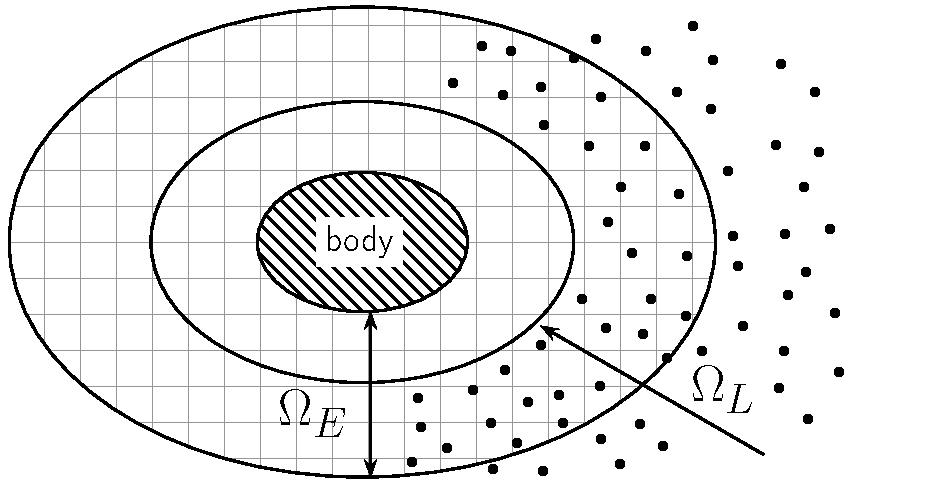
\includegraphics[width=0.6\linewidth]{figures/introduction/domainDecomposition_typical_type2.pdf}
		\caption{Standard domain decomposition using Schwartz iteration for coupling the two methods. Eulerian subdomain $\Omega_E$ (near the body), and Lagrangian subdomain $\Omega_L$ (away from the body). Figure is based on Guermond (2000) \cite{Guermond2000a}}.
		\label{fig:domainDecomposition}
	\end{figure}

\subsection{Simple coupling strategy}
This approach will be referred to as the \indexAcron{Simple Coupling Strategy}{SCS}. It is simpler than the Schwartz iterative method, as no iteration is needed for the coupling procedure. The basic algorithm consists of solving the vortex method in the full fluid domain using a relatively coarse resolution on the near-wall region. Then we use the grid solver in the near-wall region to capture the detailed features of the boundary layer and transfer the vorticity field in this region to the vortex particles, figure \ref{fig:domainDecomposition_daenick}. Therefore, the grid solver essentially acts as the correction for the under-resolved regions of the Lagrangian method. The functionality of this strategy has been demonstrated by Daeninck and was found to be significantly faster than the Schwartz coupling strategy. The features of the simple coupling strategy can summarized as follows:

	\begin{itemize}
	\item Eulerian method is used to resolve the near-wall region, at the Eulerian subdomain $\Omega_E$, enabling it to capture important features of the boundary layer (such as flow separation) with great accuracy.
	
	\item Lagrangian method is used to capture the wake, at the Lagrangian subdomain $\Omega_L$, and to efficiently evolve the wake.
	
	\item The accurate solution of the Eulerian subdomain is transfered to the Lagrangian subdomain according to the coupling algorithm of Daeninck \cite{Daeninck2006} and Stock \cite{Stock2010a}. In addition to their algorithm, a correction in done on the transfer to ensure conservation of circulation.
	
	\item The boundary conditions for the Eulerian subdomain are retrieved from the Lagrangian subdomain.
	\end{itemize}

	\begin{figure}[!t]
		\centering
		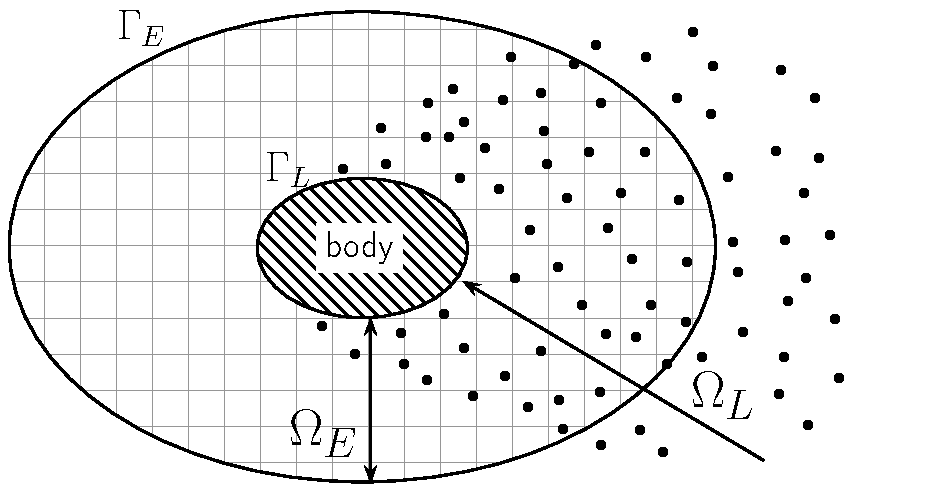
\includegraphics[width=0.6\linewidth]{figures/introduction/domainDecomposition_daenick_type2.pdf}
		\caption{Modified domain decomposition \underline{without} Schwartz alternating method. Lagrangian subdomain extends up to the surface of the body. Figure is based on Daeninck (2006) \cite{Daeninck2006}.}
		\label{fig:domainDecomposition_daenick}
	\end{figure}

The algorithm to the \printAcron{Simple Coupling Strategy}{SCS} follows from Daeninck's doctoral thesis, \cite{Daeninck2006}. Figure \ref{fig:flowchart_simpleCoupling} shows the overview to the algorithm and can be summarized as follows:

	\begin{enumerate}
	\item \textbf{Correct Lagrangian:} Use the solution of the Eulerian subdomain $\Omega_E$ (in the near-wall region) to correct the solution of the Lagrangian subdomain $\Omega_L$, that is overlapping the Eulerian subdomain, ensuring that the \textit{circulation is conserved}.  
	
	\item \textbf{Evolve Lagrangian:} With the modified solution, evolve the Lagrangian solution from time step $t_n$ to next time step $t_{n+1}$.
	
	\item \textbf{Determine Eulerian boundary conditions:} Use the Lagrangian solution of time $t_{n+1}$ to determine the boundary conditions of the Eulerian subdomain at $t_{n+1}$.
	
	\item \textbf{Evolve Eulerian:} With the boundary condition, evolve the Eulerian solution from $t_n$ to $t_{n+1}$.
	\end{enumerate}
	
This is the basic approach for coupling the Eulerian method in the Eulerian subdomain $\Omega_E$ with the Lagrangian method in the Lagrangian subdomain $\Omega_L$ without the iterative Schwartz algorithm. 

Furthermore, the SCS handles the Lagrangian boundary condition differently from the classic hybrid method. Typically during the evolution process of the Lagrangian subdomain, the shedding of the vorticity is also defined in the Lagrangian method. However, in our coupling strategy, the Lagrangian method is under-resolved at the boundary and cannot be used to resolve the vorticity flux at the body. Instead, we use the Eulerian method to resolve the boundary, and the Eulerian method acts as the vorticity generator for the Lagrangian method. However, there are some assumptions that we must satisfy, for this coupling strategy to be valid:

	\begin{itemize}
	\item At $t_n$ before the evolution of both method to $t_{n+1}$, the Lagrangian solution matches Eulerian solution at the boundary of the near-wall region.
	\item After the evolution to $t_{n+1}$, the deviation of the Lagrangian solution (due to lack of vorticity flux at Lagrangian boundary), should be minimal.
	\item Even though the Lagrangian subdomain is under-resolved in the near-wall region, it should be able to provide accurate boundary conditions for the Eulerian external boundary.
	\end{itemize}
	
	\begin{figure}[!t]
		\centering
		\begin{tikzpicture}
			[node distance=.8cm, start chain=going below,]
			\node[punktchain, join] (correct) {Correct the \\Lagrangian subdomain};
		    \node[punktchain, join] (evolveL) {Evolve the Lagrangian solution};
		    \node[punktchain, join] (bcE)     {Determine the \\Eulerian boundary conditions};
		    \node[punktchain, join] (evolveE) {Evolve the Eulerian solution};
		\end{tikzpicture}
		\caption{Flowchart of the simple coupling strategy. The flowchart shows the procedure to evolve both methods from $t_n$ to $t_{n+1}$.}
		\label{fig:flowchart_simpleCoupling}
	\end{figure}

\section{Verification and Validation Test Cases}
\label{sec:vavtc}
In order to assess the accuracy of this hybrid formulation, the following test cases haven been used:

	\begin{description}
	\item[Lamb-Oseen vortex] \cite{Lamb1993} \cite{Tryggeson2007} \hfill\\
	Lamb-Oseen vortex test case is an analytical solution derived from the NS equation, and is a test case for unbounded flow (without any wall). This is the first model that will be used to validate the Lagrangian method and Eulerian method separately. As it describes an unbounded flow, we do not need to concern with the vorticity generation problem. This helps us focus on just the evolution of the vorticity field.
	\item[Clercx-Bruneau dipole] \cite{Clercx2006a}\hfill\\
	The Clercx-Bruneau dipole test case is the simple case of a colliding dipole with a wall. This test case will be used to verify and validate the coupling of the Eulerian and the Lagrangian method in the presence of a solid wall. This test cases focuses on the interaction of vorticity with the wall making it ideal to verify and validate the proper generation of vorticity and its transfer to the Lagrangian subdomain.
	\item[Impulsively started cylinder] \cite{Koumoutsakos1995a} \cite{Chang1991} \cite{Braza1986} \cite{Lecointe1984}\hfill\\
	The impulsively started cylinder test case is used to analyze the forces acting on the cylinder. This test case is used to verify and validate the lift and drag evolution of the cylinder exposed to free-stream flow.
	\item[Elliptic Airfoil] \cite{Nair1997a}\hfill\\
	The elliptic airfoil test case focuses on the flow separation past a lifting body. The elliptic airfoil is pitched at high angle of attack and the flow past the airfoil is comparatively unsteady and undergoes phenomena such as laminar separation bubble, flow separation and karman vortex shedding from the trailing edge of the airfoil. This helps us ensure the coupling strategy is accurate for complex flow phenomena.
	\end{description}

%\todo{add picture here}
%\section{Methodology}
%The initial steps of the development of the hybrid vortex method is as follows:
%
%	\begin{enumerate}
%	\item Develop the vortex particle method
%	\item Validate the vortex particle method against a Lamb-Oseen convection test case.
%	\item Develop the vortex panel method to deal with the boundaries for the vortex particle calculation. 
%	\item Validate the vortex panel method by solving a potential flow around a cylinder.
%	\item Develop the grid solver that is based on the Finite Element method. 
%	\item Validate the grid solver against test cases: impulsively starting cylinder, dipole-Wall interaction.
%	\end{enumerate}
%
%Once all the components have been validated, the methods will be coupled and validated against similar test cases.
%
%	\begin{enumerate}
%	\setcounter{enumi}{6}
%	\item Couple vortex particle, vortex panel and grid solver together.
%	\item Validate the hybrid method with test cases provide from literature.
%%	\item Introduce more complicated phenomenons: multiple geometry (i.e multiple grid meshes) and moving boundaries, if it feasible in the constraints of a master thesis.
%	\end{enumerate}
%
%%If the coupled solver has been validated with the test cases, the final step will be to simulated the flow around a VAWT and investigating the performance vs. numerical and experimental data.

\section{Thesis Outline}

\begin{description}
\item[Ch. 2 \qquad Lagrangian Subdomain: Vortex Particle Method]\hfill\\
The chapter introduces the vortex particle method used to solve the Lagrangian subdomain of the hybrid method. The chapters introduces the concept of vortex blobs for discretizing the vorticity in the fluid and vortex panels for discretizing the wall-bounded vorticity. The chapter concludes with a verification and validation of the described Lagrangian method with the help of the Lamb-Oseen vortex test case.

\item[Ch. 3 \qquad Eulerian Subdomain: Finite Element Method]\hfill\\
The chapter introduces the finite element method used to solve the Eulerian subdomain of the hybrid method. We investigate the methodology for solving the incompressible Navier-Stokes equations using the finite element approach. The chapter concludes with a verification and validation of the described Eulerian method with the help of Lamb-Oseen vortex test case, impulsively started cylinder test case at $Re=550$ of Koumoutsakos and Leonard \cite{Koumoutsakos1995a}, and the Clercx-Bruneau dipole collision of Clercx and Bruneau \cite{Clercx2006a}.

\item[Ch. 4 \qquad Hybrid Eulerian-Lagrangian Vortex Particle Method]\hfill\\
The chapter introduces the hybrid Eulerian-Lagrangian vortex particle method. We investigate the methodology for coupling the Eulerian subdomain and the Lagrangian subdomain. This chapter highlights the modification we implemented to the coupling strategy used by Daeninck \cite{Daeninck2006} and Stock \cite{Stock2010a}.

\item[Ch. 5 \qquad Introduction to the Hybrid Solver: pHyFlow]\hfill\\
The chapter introduces \texttt{pHyFlow}, the python based hybrid solver. The chapter gives an overview of the program structure and the class hierarchy.

\item[Ch. 6 \qquad Verification and Validation of the Hybrid Method]\hfill\\
The chapter focuses on the verification and the validation of the hybrid method. We use the test cases described in section \ref{sec:vavtc}, to achieve this.

\end{description}

%\todo{To be done at the end}

%\section{Research question}
%\label{sec:ResearchQuestion}
%
%\section{Research objective}
%\label{sec:ResearchObjective}
%
%\section{Importance of study}
%
%\section{Scope of thesis}
%\label{sec:scope}
%
%\section{Structure of the report}
%\label{sec:Structure of the report}

